\documentclass[12pt]{article}
\usepackage{mathrsfs}
\usepackage{amsmath,amssymb}
\usepackage{graphicx}
\usepackage[utf8]{inputenc}
\usepackage{amsthm}
\usepackage{tkz-berge}
\usepackage{pgf}
\usepackage{xcolor}
\usepackage{algorithm}
\usepackage{caption}
\usepackage{multicol}
\usepackage{array}
\usepackage[noend]{algpseudocode}
\newcommand{\Term}{Winter 2019}
\newcommand{\Course}{104.272 Discrete Mathematics, Group 1}

\newcommand{\Assignment}{7. Exercise}
\newcommand{\DueDate}{ 27 November, 2019 }

\usepackage[body={6in,9in}]{geometry}



\begin{document}
Hugo \textit{Rincon Galeana}
\begin{center}

\textbf{TU Wien, \Term} \\
\textbf{\Course} (Professor Gittenberger) \\
\textbf{\Assignment, Due \DueDate}
\end{center}


%%%%%%%%%%%%%%%%%%%%%%%%%%%%%%%%%%%%%%%%%%%%%%%%%%%%%%%%%%%%%%%%%%%%%%%%
%% *****      Type your answers after the "\soln" commands      ***** %%
%%%%%%%%%%%%%%%%%%%%%%%%%%%%%%%%%%%%%%%%%%%%%%%%%%%%%%%%%%%%%%%%%%%%%%%%
\begin{enumerate}
    \setcounter{enumi}{60}
    \item A derangement is a permutation without any fixed point. Determine the exponential generating function $\displaystyle\sum\limits_{n \geq 0} \frac{d_n}{n!} z^n$, where $d_n$ is the number of derangements of $\{1,2,\ldots,n\}$.
    
    Then show that
    
    $$d_n = n!\displaystyle\sum\limits_{k=0}^{n} (-1)^k \frac{1}{k!}$$
    
    \begin{proof}
    Notice that a permutation $\mathcal{P}$ partitions its elements into fixed points and non fixed points. Therefore, we can view a permutation as a partitional product of a derangement and the identity permutation.
    
    Then $\mathcal{P} = \mathcal{D} \star \mathcal{I}$.
    
    The symbolic method yields the result $\hat P(z) = \hat D(Z) \cdot \hat I (z)$.
    
    Notice that $\hat P(z) = \displaystyle \sum \limits_{n\geq 0} \frac{n!}{n!} z^n = \displaystyle \sum \limits_{n\geq 0} z^ n = \displaystyle\frac{1}{1-z}$. 
    
    Notice also that $\hat I(z) = \displaystyle \sum \limits_{n\geq 0} \frac{z^n}{n!} = e^x$.
    
    It follows that $\hat D(z) = e^{-z} \cdot \frac{1}{1-z}$
    \end{proof}
    
    \item An involution is a permutation $\pi$ such that $\pi \circ \pi = \textrm {id}_M$ where $M = \{1,2,\ldots, n\}$ Let $\mathcal I$ be the set of involutions. Determine the exponential generating function $I(z)$ of $\mathcal I$.
    
    \begin{proof}
        Notice that an involution consists of a product of cycles of length 2 and 1. Simply notice that if $x$ is not a fixed point, then $x \mapsto \pi(x) \mapsto x$ which is a cycle of length 2.
        
        Notice then, that an involution is a set of size $n$ made of cycles of size 2 or 1. This leads to the following combinatorial construction:
        
        $$ \mathcal{I} = SET ( \mathcal{F} + \mathcal{P})$$
        
        Where $\mathcal I$ is an involution, $\mathcal{F}$ is a fixed point (cycle of size 1) and $\mathcal{P}$ is a pair (cycle of length 2).
        
        Notice that there is only one possible fixed point of size 1 and only one possible pair of size 2. This implies that $\hat F (z) = z$ and $\hat P(z) = \displaystyle\frac{z^2}{2}$, are the EGFs for $\mathcal{F}$ and $\mathcal{P}$ respectively.
        
        The symbolic combinatorial method now yields the following EGF for involutions. $\hat I (z) = e^ {\displaystyle{z+\frac{z^2}{2}}}$
    \end{proof}
    
    \item Use exponential generating functions to determine the number $a_n$ of \textbf{ordered} choices of $n$ balls such that there are 2 or 4 red balls, an even number of green balls and an arbitrary number of blue balls.
    \begin{proof}
    Notice that the ordered choices of this sort can be specified as a partitional product of balls of each color. Let $\mathcal{R}, \mathcal{G}, \mathcal{B}$ be the combinatorial categories of red balls, green balls and blue balls respectively. Let $\mathcal{O}$ be the combinatorial category of ordered choices as specified previously. Notice that the following definition is provided by the problem specification.
    
    $$ \mathcal{O} = \mathcal{R} \star \mathcal{G} \star \mathcal{B}$$.
    
    Notice that since there must be either 2 or 4 red balls, then the EGF for $\mathcal{R}$ is given by
    $$ \hat{R}(z) = \displaystyle\frac{z^2}{2}+ \frac{z^4}{4!}$$
    
    And respectively $ \hat{G}(z) = \displaystyle\sum\limits_{n\geq 0} \frac{z^{2n}}{(2n)!} = \displaystyle \frac{1}{2} \displaystyle \sum \limits_{n \geq 0}[1 + (-1)^n] \cdot \frac{z^n}{n!} = \displaystyle \frac{1}{2} e^z + e^{-z}$ 
    
    Also $\hat{B} = e^z$
    
    Applying the symbolic combinatorial method yields the following equation
    
    $$\hat O (z) = \displaystyle ( \frac{z^2}{2}+ \frac{z^4}{4!})  \displaystyle \frac{1}{2} \displaystyle( e^z + e^{-z}) e^z $$
    
    $$ \hat O (z)= \displaystyle ( \frac{z^2}{2}+ \frac{z^4}{4!})  \displaystyle \frac{1}{2} \displaystyle( e^{2z} + 1)$$
    
    $$ \hat O(z) = \frac{1}{2}\displaystyle ( \frac{z^2 e ^{2z}}{2}+ \frac{z^4 e^{2z}}{4!})+  \frac{1}{2}\displaystyle ( \frac{z^2}{2}+ \frac{z^4}{4!})$$
    
    Let us recall that $\displaystyle \left [\frac{z^n}{n!} \right] \hat F \cdot  \hat G = \displaystyle \sum \limits_{k\geq 0}^{n} { n \choose k} \displaystyle \left [\frac{z^k}{k!}\right ] \hat F \cdot \left [\frac{z^{n-k}}{(n-k)!}\right ] \hat G  $
    
    Notice that since $\displaystyle\left[\frac{z^k}{k!}\right ] \frac{z^2}{2}$ is only different from $0$ when $k=2$
    and  $\displaystyle\left[\frac{z^k}{k!}\right ] \frac{z^4}{4!}$ is only different from $0$ when $k=4$, then $\displaystyle\left[\frac{z^n}{n!}\right ] \frac{z^2 e ^{2z}}{2} = {n \choose 2} 2^{n-2}$ and $\displaystyle\left[\frac{z^n}{n!}\right ] \frac{z^4 e ^{2z}}{4!} = {n \choose 4} 2^{n-4}$
    
    Therefore $O(n) = \begin{cases}
1/2 +  {n \choose 2 } 2^{n-3} +  {n \choose 4 } 2^{n-5} \textrm{ if } n= 2,4 \\
 {n \choose 2 } 2^{n-3} +  {n \choose 4 } 2^{n-5} \textrm{ otherwise}\\
\end{cases}$

\end{proof}

\item Determine all solutions of the recurrence relation:
$$ a_n -2n a_{n-1} +n(n-1)a_{n-2} = 2n \cdot n!, \quad n \geq 2,\quad a_0 = a_1 = 1$$
\textit{Hint: Use exponential generating functions}

\begin{proof}
    The recurrence relation can be rewritten as follows:
    $$ a_n - 2 {n\choose 1} a_{n-1} + 2 {n \choose 2} a_{n-2} = 2n \cdot n!$$
    
    
    Notice that using the definition for the product of EGFs yields the following equation
    
    $$\hat A(z) - 2 z \hat A(z) +  z^2 \hat A (z) = \displaystyle \sum \limits_{n \geq 2} 2n z^n $$
    
    This implies that $$ \hat A(z) (1-2z+z^2) = \displaystyle \sum \limits_{n \geq 2} 2n z^n$$
    
    This yields $$ \hat A(z) = \displaystyle \sum \limits_{n \geq 2} 2nz^n / (z-1) ^2$$
    
    It follows that $$ \hat A(z) = 2 (\frac{z}{1-z})' (1-z)^{-2}$$
    
    This implies that $\hat A(z) = 2z (1-z)^{-4} = 2z (z-1) ^ {-4}$. Applying the negative binomial theorem yields $\hat A(z) = 2z \displaystyle \sum \limits_{n\geq 1} {4+n-1 \choose n}z ^n (-1^n)  (-1^{-n})$
    Therefore $\hat A(z) = \displaystyle \sum \limits_{n \geq2} 2 {n+2 \choose n-1} z^{n} = \displaystyle \sum \limits_{n \geq2} 2 {n+2 \choose 3} z^{n}  = \displaystyle \sum \limits_{n \geq2} \frac{(n+2) (n+1) (n-1)}{3}  z^{n}$.
    
    Since $\hat A(z)$ is an EGF, then $a_n = \begin{cases} 1 \quad \textrm{ if } n = 0,1 \\ \displaystyle\frac{(n-1)(n+2)!}{3} \quad \textrm{otherwise}\end{cases}$
    

\end{proof}
    \item Let $S_{n,k}$ be the Stirling numbers of the second kind, that is, the number of partitions of the set $\{1,2, \dots, n\}$ into $k$ (non-empty) subsets. Show the following formula:
    $$ \sum \limits_{n,k} S_{n,k} \frac{z^n}{n!}u^k = e^{u(e^z-1)}$$.
    
    \begin{proof}
        First we will compute a formula for the Stirling numbers of the second kind.
        
        Assume that $a_1 + a_2 + \ldots + a_k = n$. For now we will label each partition as $P_1, P_2, \ldots, P_k$ such that $\vert P_i \vert = a_i$, and later we will remove the labels.
        
        Notice that we can choose from ${n \choose a1}$ options for $P_1$. Now that we have picked the elements for $P_1$, we can proceed to pick the elements for $P_2$. We have ${n-a_1 \choose a_2}$ options for $P_2$ and inductively we have $$\displaystyle {n-\sum \limits_{j=1}^{i-1} a_j \choose a_i}$$
        different options for partition $P_i$. Therefore we have 
        
        $$ \prod\limits_{i=1}^{k} \displaystyle{n-\sum \limits_{j=1}^{i-1} a_j \choose a_i}$$ This corresponds to $ \displaystyle\frac{n!}{a_1! a_2! \ldots a_k!}$ (notice that expanding the product makes the rest of the terms cancel out).
        
        Therefore we have 
        \begin{equation}
          S_{n,k}=\frac{n!}{k!}(\displaystyle\sum \limits_{a_1+a_2+\ldots + a_k = n } \frac{1}{a_1! a_2! \ldots a_k!}) 
        \end{equation}
        
        We added over all possible size assignments to the sets of the partitions $P_i$, and then we remove the set labels dividing by $k!$.
        
        Now, recall that $e^z = \sum \limits_{k=0}^\infty \frac{z^k}{k!}$. This implies by substitution that $e^{u(e^z -1)} = \sum \limits_{k=0}^\infty \frac{[u (e^z-1)]^k}{k!} = \sum \limits_{k=0}^\infty \frac{u^k}{k!} [e^z-1]^k $. Notice that $e^z-1 = \sum \limits_{n = 1}^{\infty} \frac{z^n}{n!}$. We can use this information to compute $[e^z-1]^k$ as a Cauchy product. 
        
        It follows that $[z^n](e^z-1)^k = \displaystyle \sum \limits_{a_1+a_2+\ldots+ a_k =n} \frac{1}{a_1! a_2! \ldots a_k!} = \frac{k!}{n!}S_{n,k}$. This implies that $\sum \limits_{k=0}^\infty \frac{u^k}{k!} [e^z-1]^k = \displaystyle\sum \limits_{k=0}^\infty \sum \limits_{n=0}^k   S_{n,k} \frac{u^k}{n!} z^n $
    \end{proof}
    
    \item Prove the following representation for the Stirling numbers of the second kind:
    
    $$ S_{n,k} = \frac{1}{k!} \displaystyle \sum \limits_{j=0}^{k}(-1)^k {k \choose j} j^n$$
    
    \textit{Remark: compute first the generating function for $\displaystyle \sum \limits_{n=0}^{\infty} S_{n,k} \frac{z^n}{n!} = \frac{(e^z-1)^k}{k!}$}
    
    \begin{proof}
    Notice that $(e^z-1) = \displaystyle \sum_{k=1}^{\infty} \frac{z^n}{n!}$, then $\frac{(e^z-1)^k}{k!} = \displaystyle\frac{1}{k!} \sum \limits_{\sum a_i = n} \frac{1}{a_1! a_2 ! \ldots a_n!} z^n = \displaystyle \sum \limits_{n=0}^ {\infty}S_{n,k} \frac{z^n}{n!}$
    
    From the binomial theorem, it follows that $(e^z -1)^ k = \displaystyle \sum\limits_{j=0}^{k} (-1)^{k-j}{k \choose j}e^{zj} = \displaystyle \sum \limits_{j=0}^{k} (-1)^{k-j}{k \choose j} \displaystyle\sum_{n=0}^{\infty}\frac{z^n j^n}{n!} $. Since $\frac{(e^z-1)^k}{k!}= \displaystyle \sum_{n=0}^{\infty}\displaystyle  \frac{1}{k!}\sum \limits_{j=0}^{k} (-1)^{k-j}{k \choose j} j^n\frac{z^n }{n!} $ is the EGF for $S_{n,k}$ , it follows that $S_{n,k} = \displaystyle\frac{1}{k!}\sum \limits_{j=0}^{k} (-1)^{k-j}{k \choose j} j^n$
    \end{proof}
    
    \item Let $P$ be the set of all divisors of 12. Determine the Möbius function of $(P, \; \vert \;)$
    \begin{proof}
        
    
    Notice that $(\mathbb{N}^+ , \quad \vert ) \cong (\mathbb{N} \times \mathbb{N} \times \ldots , \leq)$ since every positive integer can be factorized uniquely as a product of powers of primes with only finitely many greater than 0 powers. Notice then that $a = p_1^{a_1}p_2^{a_2} p_3^{a_3} \ldots p_n^{a_n} \; \vert \; b = p_1^{b_1} p_2^{b_2} \ldots p_n^{b_n}$ if and only if $a_i \leq b_i$ for all $i \in \{1, \ldots, n\}$.
    
    Therefore the Möbius function for the divisibility order can be computed as a product of Möbius functions with respect to the usual order in $\mathbb{N}$.  $$\mu_{\vert}(a,b) = \displaystyle \prod\limits_{i=1}^{n}\mu_{\leq}(a_i,b_i)$$
    
    Recall that the Möbius function for the usual order in $\mathbb{N}$ is given by 
    $$ \mu_{\leq}(n,m)= \begin{cases} 0 &\textrm{ if } n>m \vee m \geq n+2 \\
                                      1 &\textrm{ if } n= m \\ 
                                     -1 &\textrm{ if }m = n+1    \end{cases} $$
    Since $\mu(n,n) = \delta(n,n) = 1$, $\mu(n,n+1)+\mu(n+1,n+1) = \delta(n,n+1)= 0 $ then $\mu(n,n+1) = -1$ and notice also that $\delta(n,n+2) = 0 = \delta(n+1,n+2) + \mu(n,n+2)  = \mu(n,n+2)$. Inductively $\mu(n,m) = 0$ for any $n+2 \leq m$.
    
    Notice that this implies that $$\mu_{ \vert } (a,b) = \begin{cases} 0 & \textrm{if } a  \not \vert \; b \vee b/a = p^{2} z ,\; p \in \mathcal P, z \in \mathbb{N}^+ \\
    (-1)^k & \textrm{ if }  b/a = p_1 p_2 \ldots p_k, p_i \in \mathcal{P}
                        \end{cases}$$
    
    Where $\mathcal{P}$ is the set of positive prime numbers.
    
    Notice that since divisibility is transitive then if $a \; \vert \; b \;\vert \; 12$ then $a \;\vert \; 12$. This implies that the Möbius function for $(div(12), \; \vert \;)$ is a restriction of the Möbius function for $(\mathbb{N}^+, \; \vert \; )$. Therefore it has the same definition.
    \end{proof}
    \item Let $(P,\leq)$ be the poset defined by $P=\{0,1,2,3,4\}$ and the three relations
    $$ 0 \leq 1 \leq 4, \quad 0 \leq 2 \leq 4, \quad 0 \leq 3 \leq 4$$
    
    Compute all values $\mu(x,y)$ for $x,y \in P$
    \begin{proof}
        
    
    $\mu(n,n) = 1, \mu(1,4) = \mu(2,4) = \mu (3,4) = \mu(0,1) = \mu(0,2) = \mu(0,3) = -1$
    
    Also notice that $\delta(0,4) = 0 = \displaystyle \sum \limits_{z \in [0,4]}\mu(z,4) = \mu(0,4)-3+1$ this implies that $\mu(0,4) = 2$
    
    $\mu(n,m) = 0 $ in all the remaining cases.
    \end{proof}
    \item Let $(P_1, \leq _1)$ and $(P_2, \leq_2)$ be two locally finite posets and $(P, \leq)$ be defined by $P = P_1 \times P_2$ and for $(a,x),(b,x) \in P:$
    
    $$ (a,x) \leq (b,y) \Leftrightarrow a \leq_1 b \wedge x \leq_2 y$$
    
    Show that $(P, \leq)$ is a poset and that the Möbius functions of $P,P_1$ and $P_2$ satisfy $$\mu_P((a,x),(b,y)) = \mu_{P_1}(a,b) \cdot \mu_{P_2}(x,y)$$
    
    \begin{proof}
    
        \textbf{ $\leq$ is Reflexive}:
        
        Let $(a,b) \in P$. Since $P_1$ and $P_2$ are posets, then $a\leq_1 a \wedge b \leq_2 b$. From the definition $(a,b) \leq (a,b)$.
        
        \textbf{ $\leq$ is Antisymmetric}:
        
        Assume that $(a,b) \leq (c,d) \wedge (c,d) \leq (a,b)$. From the definition of $\leq$, it follows that $a \leq_1 c \leq_1 a \wedge b \leq_2 d \leq_2 b$. Since $P_1$ and $P_2$ are posets, then it follows that $a=c \wedge b=d$. Therefore $(a,b) = (c,d)$, and $\leq $ is antisymmetric.
        
        \textbf{ $\leq$ is Transitive}:
        
        Assume that $(a_1,b_1) \leq (a_2,b_2) \leq (a_3,b_3)$. From the definition, then $a_1 \leq_1 a_2 \leq_1 a_3 \wedge b_1 \leq_2 b_2 \leq_2 b_3$. Since $P_1$ and $P_2$ are posets, it follows that $a_1 \leq_1 a_3 \wedge b_1 \leq_2 b_3.$ From the definition, it follows that $(a_1,b_1) \leq (a_3,b_3)$.
        
        This proves that $(P,\leq) $ is a poset.
        
        Notice that the Kronecker delta for $P $ , $\delta_P = (\delta_{P_1} \circ \pi_1) \cdot (\delta_{P_2} \circ \pi_2)$ where $\pi_1$ and $\pi_2$ are the projections on the first and second coordinate respectively.
        
        Now notice that $\delta( (a,b) , (c,d)) = \displaystyle\sum\limits_{(x,y) \in [(a,b),(c,d)]} \mu_{P} ((x,y),(c,d))$
        
        On the other hand, $\delta( (a,b) , (c,d)) = \delta( a, c) \cdot \delta(b,d) = \displaystyle\sum \limits_{x \in [a,c]} \mu_{P_1}(x,c) \displaystyle\sum \limits_{y \in [b,d]} \mu_{P_2}(y,d) = \displaystyle \sum \limits_{(x,y) \in [(a,b),(c,d)]} \mu_{P_1}(x,c) \cdot \mu_{P_2}(y,d)$
        
        Applying the first equation yields 
        
        $$\displaystyle \displaystyle\sum\limits_{(x,y) \in [(a,b),(c,d)]} \mu_{P} ((x,y),(c,d)) = \displaystyle \sum \limits_{(x,y) \in [(a,b),(c,d)]} \mu_{P_1}(x,c) \cdot \mu_{P_2}(y,d)$$
        
        Since we are only considering locally finite posets, then it can be shown by induction over $\vert [(a,b),(c,d)] \vert $ that $\mu_P((x,y), (c,d)) = \mu_{P_1}(x,c) \cdot \mu_{P_2}(y,d)$ for any $(x,y) \in [(a,b),(c,d)]$
        
        $$\mu_P((a,x),(b,y)) = \mu_{P_1}(a,b) \cdot \mu_{P_2}(x,y)$$
        \end{proof}
        
        \item Draw the Hasse diagran of the poset $P:= ( 2^{\{1,2,3\}}, \supseteq)$.
        
        Let now $A_1, A_2, A_3 \subseteq M$. Use Möbius inversion on the poset $P$ to show the following inclusion-exclusion principle
        $$ \vert M \setminus \bigcup\limits_i A_i \vert  = \vert M \vert - \displaystyle \sum \limits_i \vert A_i \vert + \displaystyle \sum_{i \neq j}  \vert A_i \cap A_j \vert - \vert A_1\cap A_2 \cap A_3 \vert$$
        
        \begin{proof}
            
        \end{proof}
        \begin{center}
        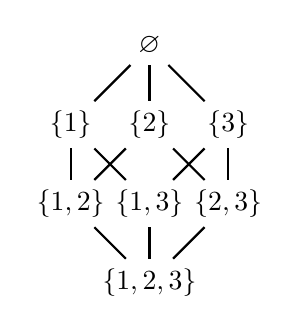
\begin{tikzpicture}
        \node (top) at (0,0) {$\varnothing$};
        \node (s1) at (-1,-1)  {$\{1\}$};
        \node (s2) at (0,-1) {$\{2\}$};
        \node (s3) at (1,-1) {$\{3\}$};
        \node (s12) at (-1,-2) {$\{1,2\}$};
        \node (s13) at (0,-2) {$\{1,3\}$};
        \node (s23) at (1,-2) {$\{2,3\}$};
        \node (bot) at (0,-3) {$\{1,2,3\}$};
        \draw [black,  thick] (top) -- (s1);
        \draw [black,  thick] (top) -- (s2);
        \draw [black,  thick] (top) -- (s3);
        
        \draw [black,  thick] (s1) -- (s12);
        \draw [black,  thick] (s1) -- (s13);
        \draw [black,  thick] (s2) -- (s12);
        \draw [black,  thick] (s2) -- (s23);
        \draw [black,  thick] (s3) -- (s13);
        \draw [black,  thick] (s3) -- (s23);
        
        \draw [black,  thick] (bot) -- (s23);
        \draw [black,  thick] (bot) -- (s13);
        \draw [black,  thick] (bot) -- (s12);
        
    \end{tikzpicture}
    \end{center}
    
    We consider the function $f: P \rightarrow \mathbb{R}, f(I) = \vert M \cap \bigcap\limits_{i \in I}A_i \cap (\bigcap\limits_{j \notin I}M \setminus A_i)\vert $
    
    The definition for $S_f(I) = \displaystyle\sum\limits_{J \supseteq I} f(J) = \displaystyle\sum\limits_{J \supseteq I} \vert \bigcap\limits_{i \in I}A_i \cap(\bigcap\limits_{j \notin I} M \setminus A_i)\vert$.
    
    Notice that $\displaystyle\bigcup\limits_{J \supseteq I} ( M \cap \bigcap\limits_{i \in J}A_i \cap (\bigcap\limits_{j \notin J}M \setminus A_i)) = M \cap \bigcap \limits_{i\in I} A_i$ since one contention is trivial by definition and for any $x \in M \cap \displaystyle\bigcap \limits_{i \in I} A_i$, if $x \in A_j$ , then $S_x = \{ j \; \vert \; j \notin I, x \in A_j \}$. It follows that $x \in M \cap \bigcap\limits_{i \in I \cup S_x} A_i \cap (\bigcap\limits_{j \notin I \cup S_x} M \setminus A_j)$.
    
    Notice that if $J \neq Q, J \supseteq I, Q \supseteq I$, then $\hat J \cap \hat Q = \varnothing$ for $\hat J = M \cap \bigcap\limits_{i \in J}A_i \cap (\bigcap\limits_{j \notin J}M \setminus A_i) $ and $\hat Q = M \cap \bigcap\limits_{i \in Q}A_i \cap (\bigcap\limits_{j \notin Q}M \setminus A_i)$. 
    
    This shows that these are pairwise disjoint sets. Therefore $S_f(I) = \vert \bigcap\limits_{i \in I} A_i \vert$
    
    Applying the Möbius inversion theorem, then $f(\varnothing) = \vert M \setminus \bigcup\limits_{i} A_i \vert = \displaystyle \sum \limits_{J \subseteq\{1,\ldots,m\}} (-1)^{\vert J \vert} \left \vert \bigcap\limits_{j \in J}A_j \right\vert$
    
    By grouping together sets with the same cardinality we get 
    
    $$\displaystyle \sum \limits_{i=0 }^{m} \sum\limits_{\vert J \vert = i} (-1)^i \left \vert \bigcap_{j \in J } A_j\right \vert  = \vert M \vert - \vert A_1 \vert - \vert A_2 \vert \ldots - \vert A_m \vert + \vert A_1 \cap A_2\vert + \ldots$$
    \end{enumerate}
\end{document}
        
        
    
    
\end{document}